% arara: xelatex
% arara: xelatex

\documentclass[czech]{ctufit-presentation}

\usepackage{booktabs}

\graphicspath{{images/}{../images/}}

\ctufittitle{Software pro evidenci majetku}
\ctufitsubtitle{Bakalářská práce \\[0.3em] {\small Vedoucí práce: Ing.\,Jiří Mlejnek}}
\ctufitauthor{Ondřej Kopáč}
\ctufitdate{\today}
\ctufitinstitute{FIT ČVUT v Praze}

\begin{document}

% --------------------------------------------------------------------
% 1. Titulní slide
% --------------------------------------------------------------------
\begin{frame}[plain,t]
	\titlepage
\end{frame}

% --------------------------------------------------------------------
% 2. Motivace a rešerše
% --------------------------------------------------------------------
\section{Úvod}

\begin{frame}
	\frametitle{Motivace a rešerše}
	\framesubtitle{Proč vlastní řešení}
	\begin{itemize}
		\item Zadavatel: ZŠ Ústavní (Praha~8), evidence majetku v~Excelu
		\item Potřeba: inventura s~průmyslovou čtečkou, tisk etiket, offline režim
	\end{itemize}
	\vspace{0.3em}
	\begin{center}
		\footnotesize
		\setlength{\tabcolsep}{3pt}
		\resizebox{\textwidth}{!}{%
		\begin{tabular}{lccccc}
			\toprule
			& Excel & EVIDEI & Sp.\,Maj. & Snipe-IT & \textbf{Vlastní} \\
			\midrule
			Inventura s~čtečkou & -- & \checkmark & \checkmark & \checkmark & \checkmark \\
			Offline režim       & -- & \checkmark & --         & --         & \checkmark \\
			Zebra TC22          & -- & \checkmark & --         & --         & \checkmark \\
			Tisk ZPL etiket     & -- & \checkmark & --         & --         & \checkmark \\
			Cena                & 0  & vysoká     & nízká      & 0          & 0 \\
			\bottomrule
		\end{tabular}}
	\end{center}
	\vspace{0.3em}
	{\small Žádné existující řešení nepokrývá kombinaci požadavků za přijatelnou cenu.}
\end{frame}

% --------------------------------------------------------------------
% 3. Architektura systému
% --------------------------------------------------------------------
\section{Návrh}

\begin{frame}
	\frametitle{Architektura systému}
	\framesubtitle{Tři komponenty komunikující přes REST API}
	\begin{itemize}
		\item \textbf{Backend} -- Spring Boot + PostgreSQL
		\item \textbf{Webová aplikace} -- React + TypeScript + Vite
		\item \textbf{Mobilní aplikace} -- nativní Android pro Zebra TC22
		\item Autentizace JWT (access + refresh token s~rotací)
	\end{itemize}
	\begin{center}
		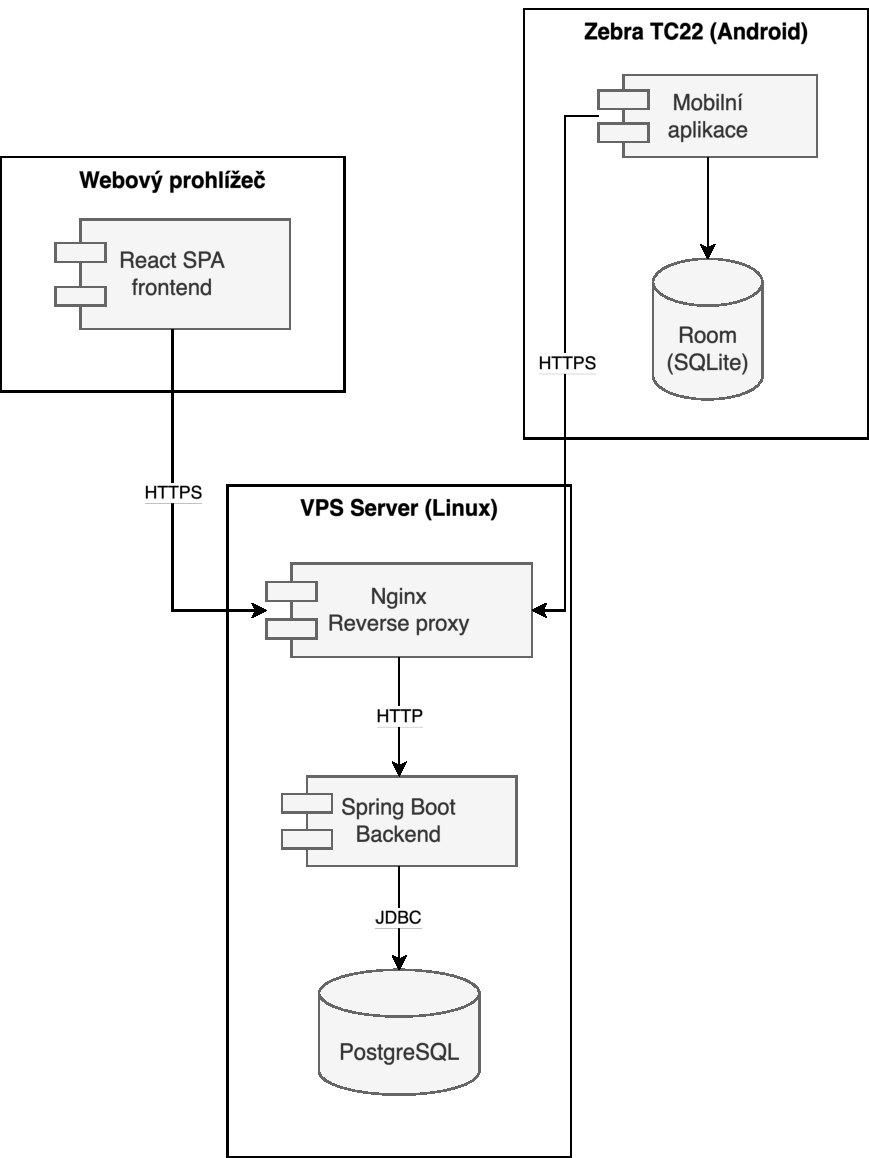
\includegraphics[width=0.95\linewidth,height=0.6\textheight,keepaspectratio]{system-architecture.pdf}
	\end{center}
\end{frame}

% --------------------------------------------------------------------
% 4. Webová aplikace
% --------------------------------------------------------------------
\section{Implementace}

\begin{frame}
	\frametitle{Webová aplikace}
	\framesubtitle{Správa karet, číselníků a~vyhodnocení inventury}
	\begin{itemize}
		\item Master-detail layout, inline editace číselníků
		\item Fulltext s~diakritikou (PostgreSQL \texttt{unaccent})
		\item Generování PDF, Excel, ZPL etiket
	\end{itemize}
	\begin{center}
		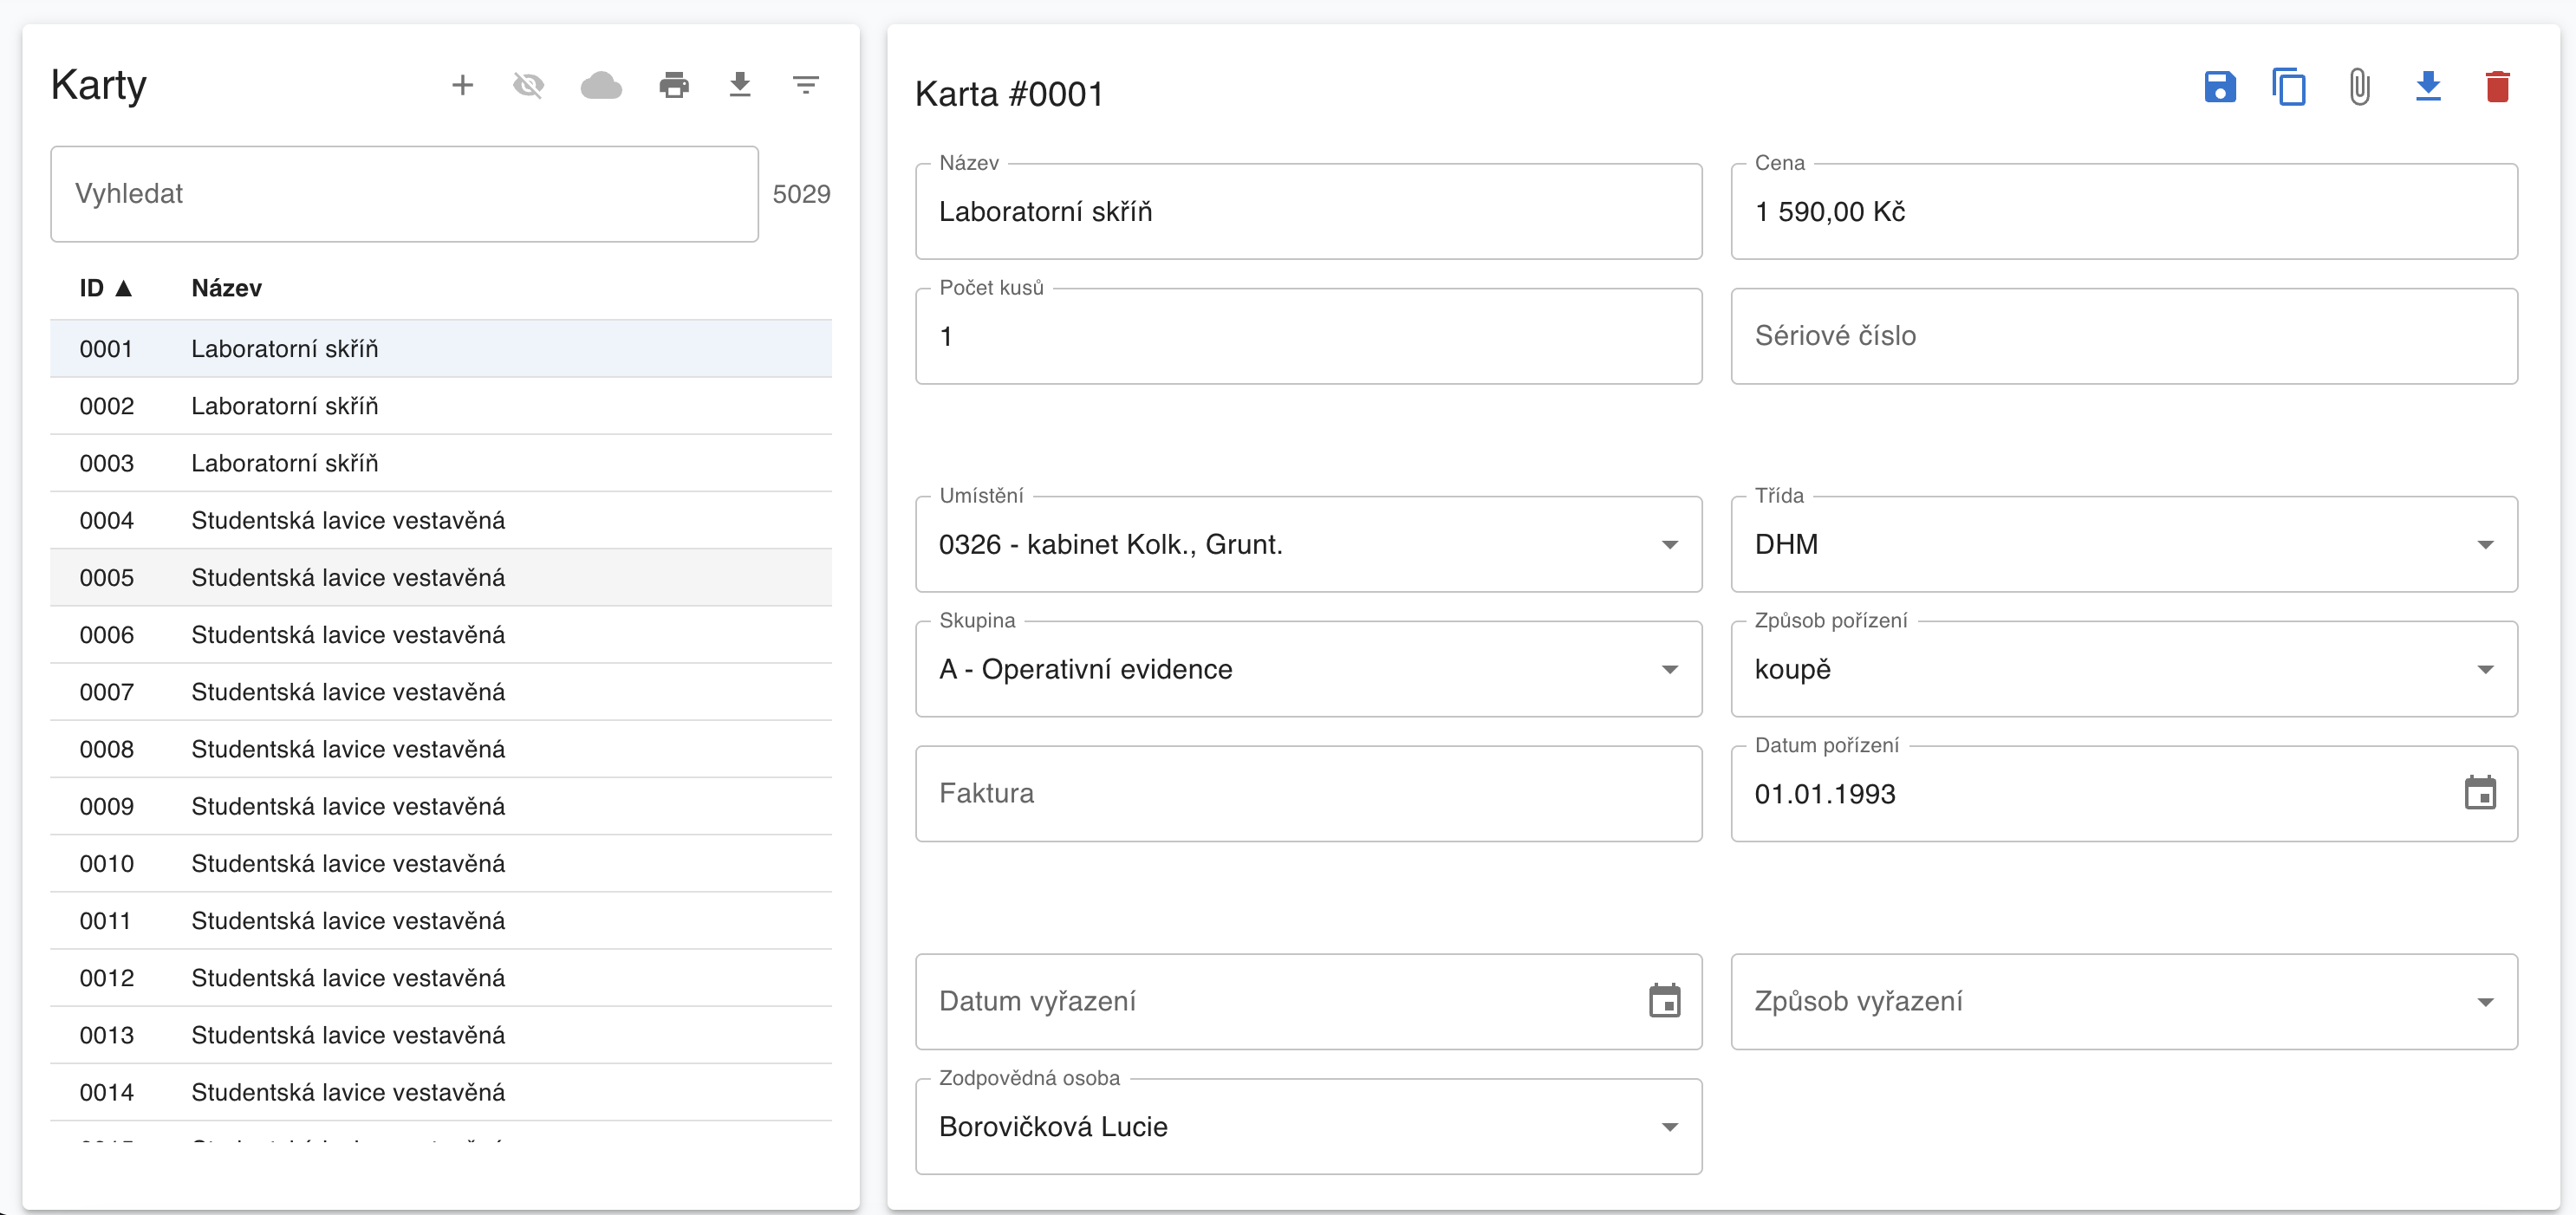
\includegraphics[width=0.85\linewidth,height=0.55\textheight,keepaspectratio]{card_page.png}
	\end{center}
\end{frame}

% --------------------------------------------------------------------
% 5. Mobilní aplikace pro Zebra
% --------------------------------------------------------------------
\begin{frame}
	\frametitle{Mobilní aplikace pro Zebra}
	\framesubtitle{Klíčový rozdíl od konkurence: offline-first}
	\begin{columns}[T]
		\column{0.65\textwidth}
		\begin{itemize}
			\item Cílové zařízení: \textbf{Zebra TC22} -- enterprise Android terminál s~vestavěnou čtečkou
			\item Nativní Android (Java), Room DB (SQLite)
			\item Šifrované úložiště přihlašovacích údajů
			\item Synchronizace dat se serverem
		\end{itemize}

		\column{0.35\textwidth}
		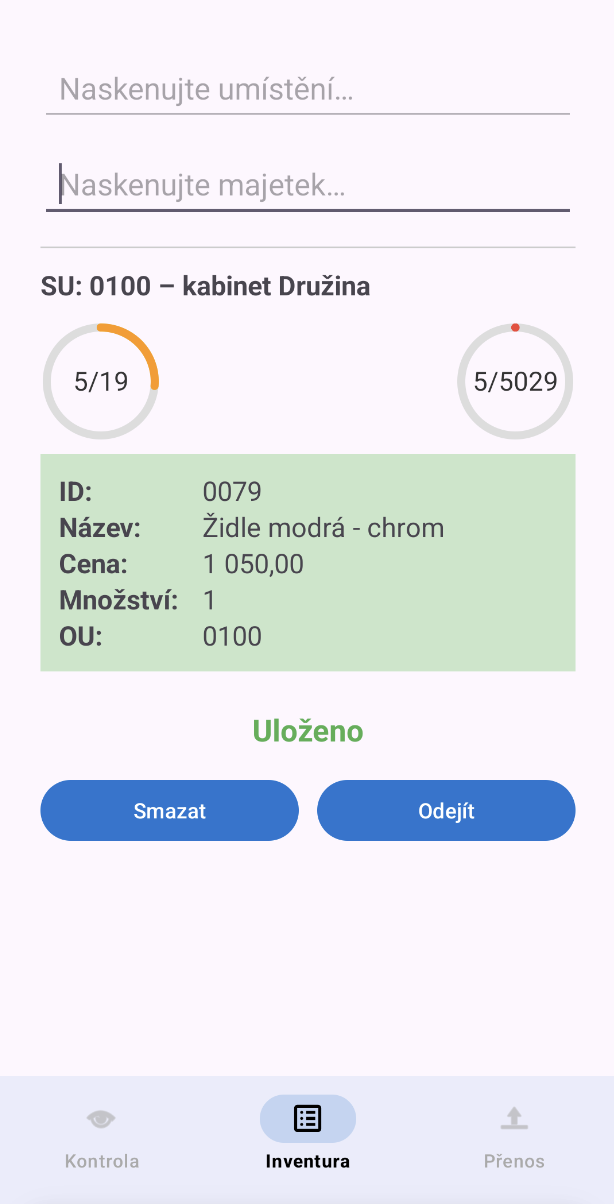
\includegraphics[width=\linewidth]{scanning_page.png}
	\end{columns}
\end{frame}

% --------------------------------------------------------------------
% 6. Inventurní proces
% --------------------------------------------------------------------
\begin{frame}
	\frametitle{Inventurní proces}
	\framesubtitle{Od skenování po promítnutí změn do databáze}
	\footnotesize
	\begin{enumerate}
		\item Stažení dat do mobilní aplikace
		\item Skenování v~terénu (offline)
		\item Synchronizace na server
		\item Vyhodnocení rozdílů
		\item Promítnutí změn do databáze
	\end{enumerate}
	\begin{center}
		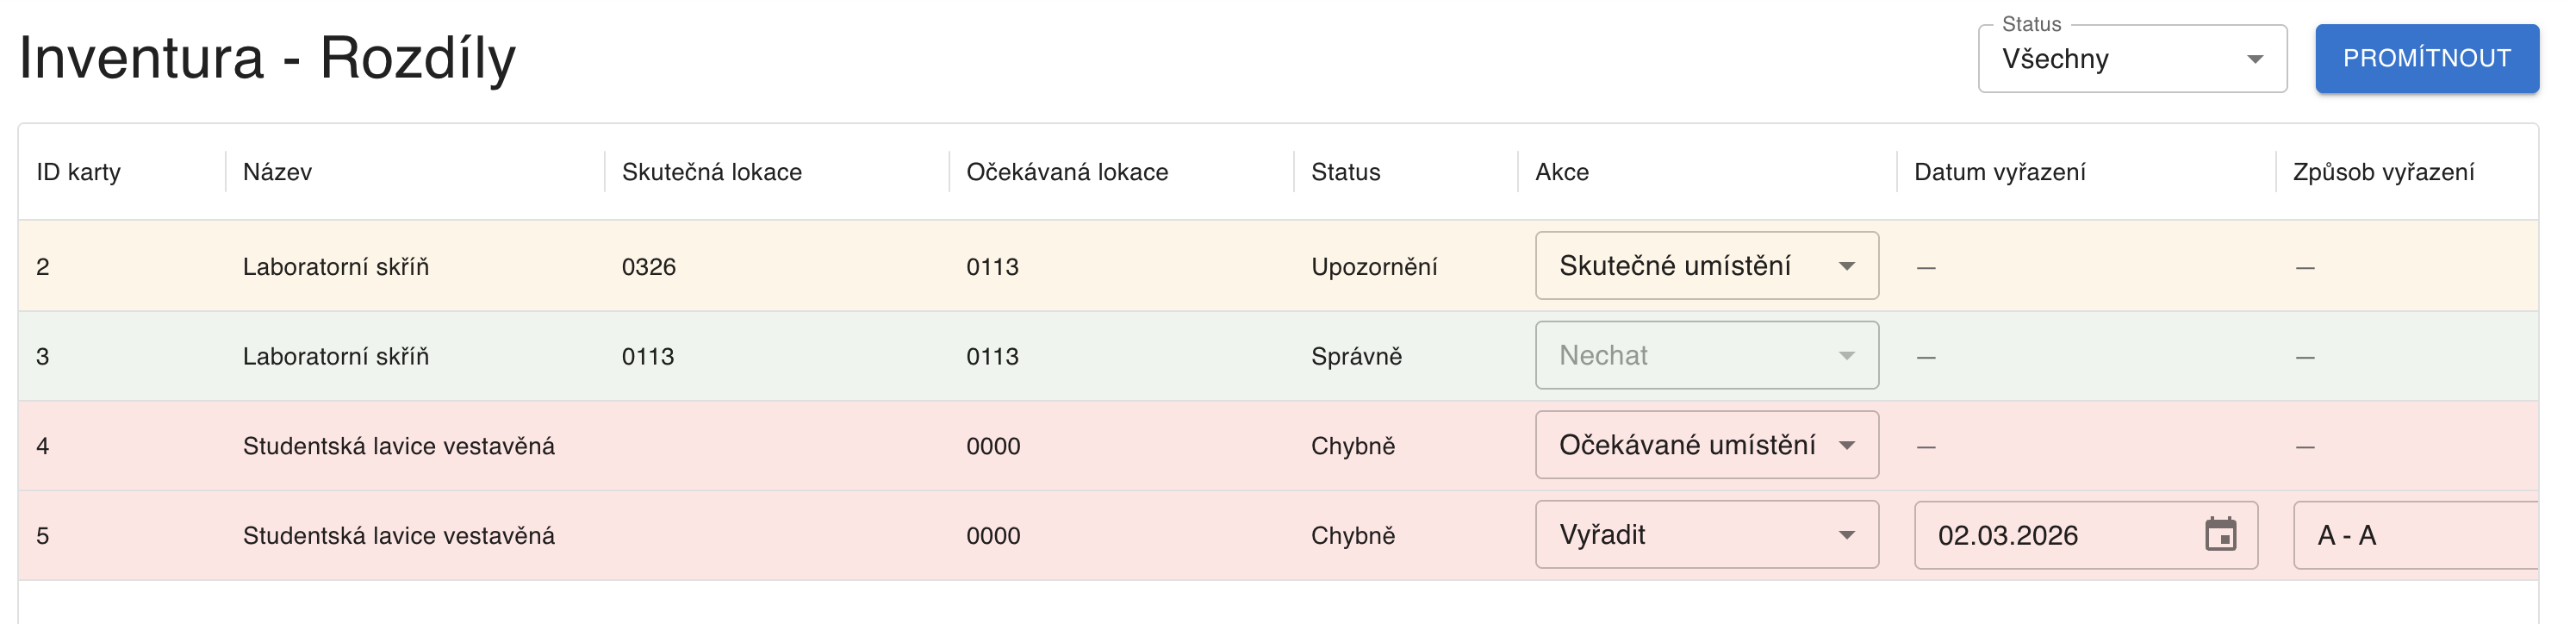
\includegraphics[width=0.95\linewidth,height=0.45\textheight,keepaspectratio]{differences_page.png}
	\end{center}
	{\footnotesize Stavy: \textcolor{green!60!black}{CORRECT} (souhlasí), \textcolor{orange}{WARN} (jiné umístění), \textcolor{red}{WRONG} (nenalezeno).}
\end{frame}

% --------------------------------------------------------------------
% 7. Testování
% --------------------------------------------------------------------
\section{Testování}

\begin{frame}
	\frametitle{Testování a kvalita kódu}
	\begin{itemize}
		\item Pokrytí testy na všech třech modulech:
			\begin{itemize}
				\item Backend -- JUnit, Mockito, MockMvc
				\item Webová aplikace -- Vitest, Testing Library
				\item Mobilní aplikace -- JUnit + instrumentované testy
			\end{itemize}
		\item Vynucené pokrytí backendu \textbf{80\,\% řádků} (JaCoCo)
		\item CI/CD: GitHub Actions + statická analýza SonarCloud
	\end{itemize}
\end{frame}

% --------------------------------------------------------------------
% 8. Nasazení a stav v praxi
% --------------------------------------------------------------------
\begin{frame}
	\frametitle{Nasazení}
	\framesubtitle{Produkční systém v~ostrém provozu}
	\begin{itemize}
		\item VPS, Linux, Nginx (HTTPS, Let's Encrypt), systemd, automatický backup PostgreSQL
		\item Automatický deploy přes GitHub Actions (manuální spouštění)
		\item Hardware: Zebra TC22 (čtečka) + Zebra ZD621d (tiskárna ZPL etiket)
		\item URL: \texttt{https://majetek.zs-ustavni.cz}
	\end{itemize}
	\vspace{0.5em}
	{\small Etiketování školy probíhá, systém je technicky připraven na první ostrou inventuru.}
\end{frame}

% --------------------------------------------------------------------
% 9. Závěr
% --------------------------------------------------------------------
\section{Závěr}

\begin{frame}
	\frametitle{Závěr}
	\begin{exampleblock}{Splněné cíle}
		Funkční i~obecné požadavky realizovány.
		Systém nasazen v~produkci pro konkrétního zadavatele.
	\end{exampleblock}
	\begin{itemize}
		\item Limity: jednouživatelská inventura, manuální distribuce APK
		\item Možnosti rozvoje: import CSV/Excel, historie změn, RFID, plánování údržby, MDM
	\end{itemize}
\end{frame}

% --------------------------------------------------------------------
% 10. Děkuji za pozornost
% --------------------------------------------------------------------
\begin{plainFrame}[colourbg]
	\plainFrameText{Děkuji za pozornost}
\end{plainFrame}

\end{document}
